%Correctness
\section{Correctness}

In this section we will look at the correctness of the translation process. Correctness for us can be described as a mapping show in Figure \ref{fig:correctness_graph1}. Expressions in our system are compiled into the program code. Expressions can be evaluated by hand ($\delta$) to produced a value. Likewise the program can be executed to produce a final value. Correctness holds in our system if the value of the evaluation ($\delta$) is the same as a value achieved by execution.

\begin{figure}[htb]
    \centering
    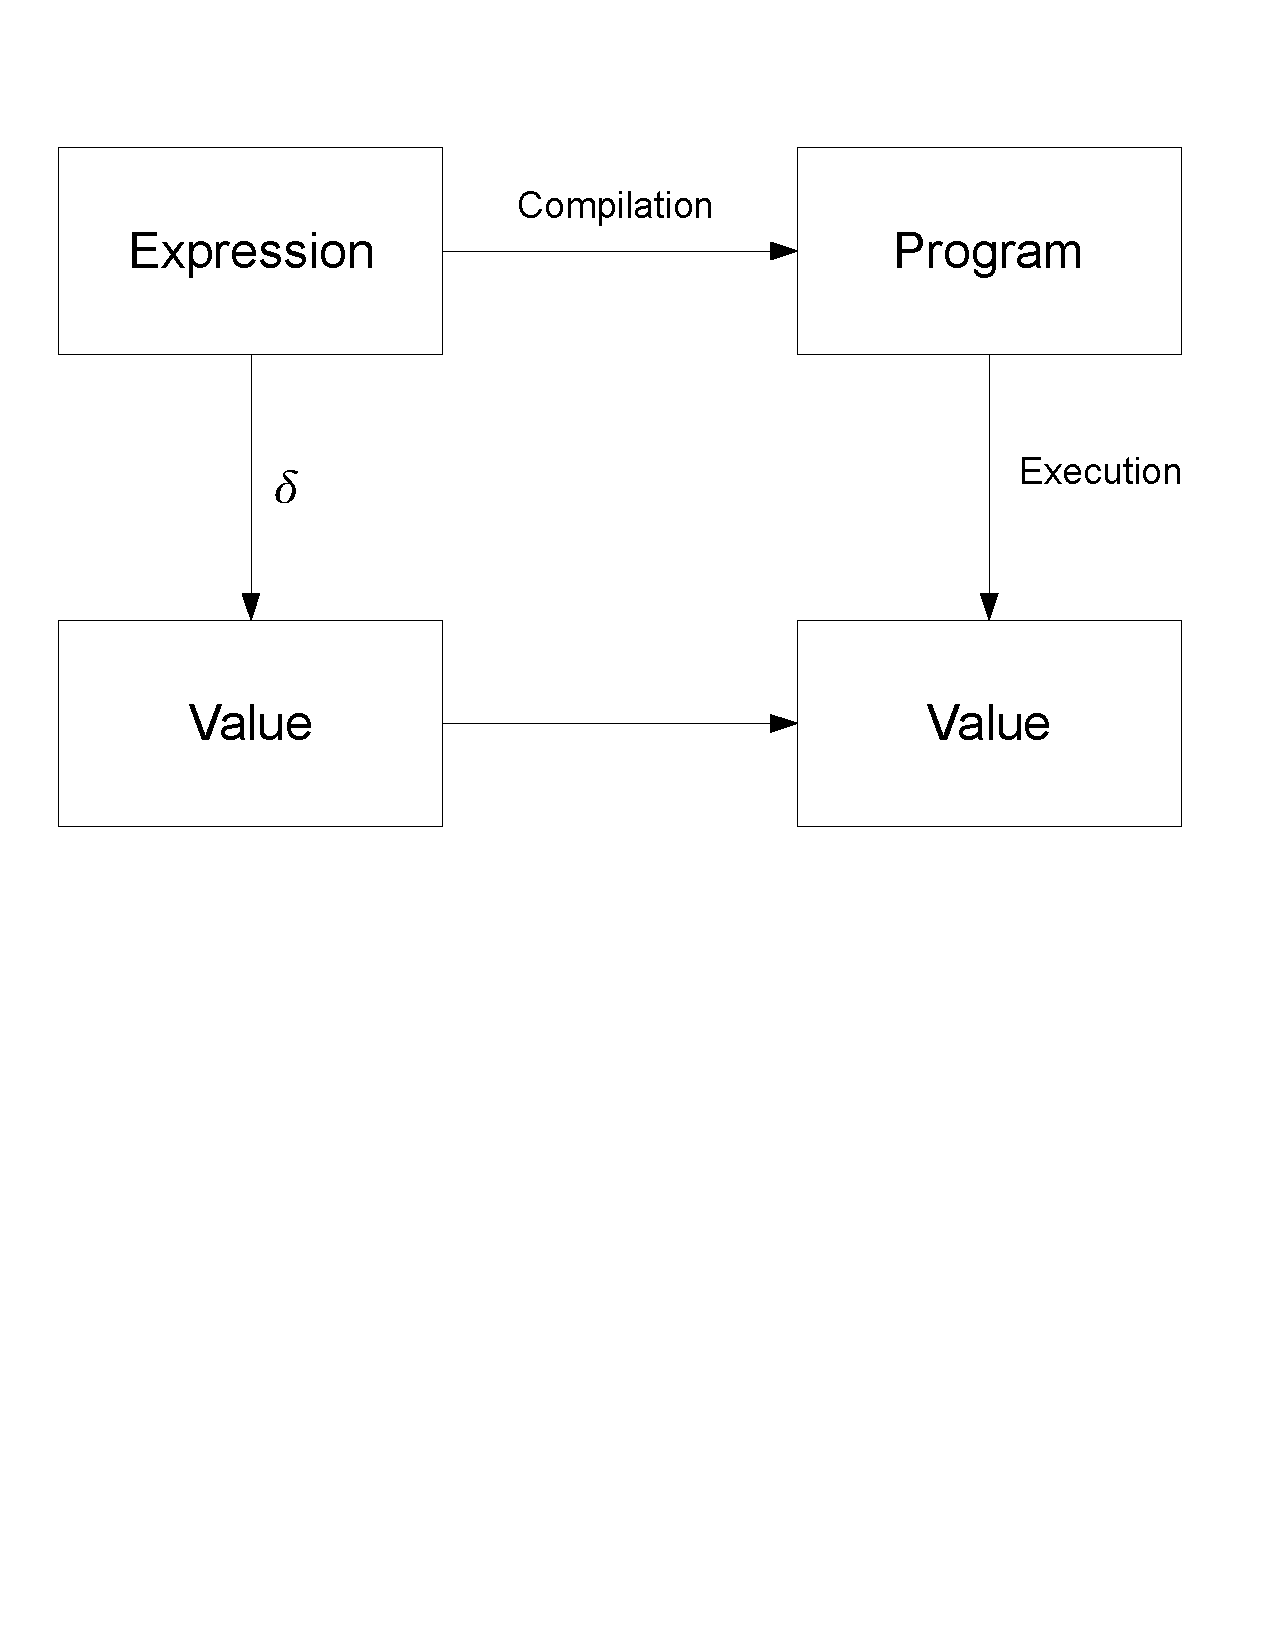
\includegraphics[trim= 10mm 120mm 10mm 10mm, clip, width=250px]{./images/correctness_graph1.pdf}
    \caption{Code Transformations}
    \label{fig:correctness_graph1}
\end{figure}

The graph structure of \plccharts is directed graph in which the constructs are discussed in detail in sections \ref{sec:statechartsyn} and \ref{sec:statechartsem}. Our tool constructs executable code from on the diagram constructs.  In addition showing the mapping for Figure \ref{fig:correctness_graph1} we also need to justify the program structure generated from an graph structure is correct. To do so we extend figure \ref{fig:correctness_graph1} to obtain figure \ref{fig:correctness_graph2} to incorporate transitions. If each Figure \ref{fig:correctness_graph1} represents an individual block than the extended Figure \ref{fig:correctness_graph2} represents the several individual blocks with the ability to transition between them.

\begin{figure}[htb]
    \centering
    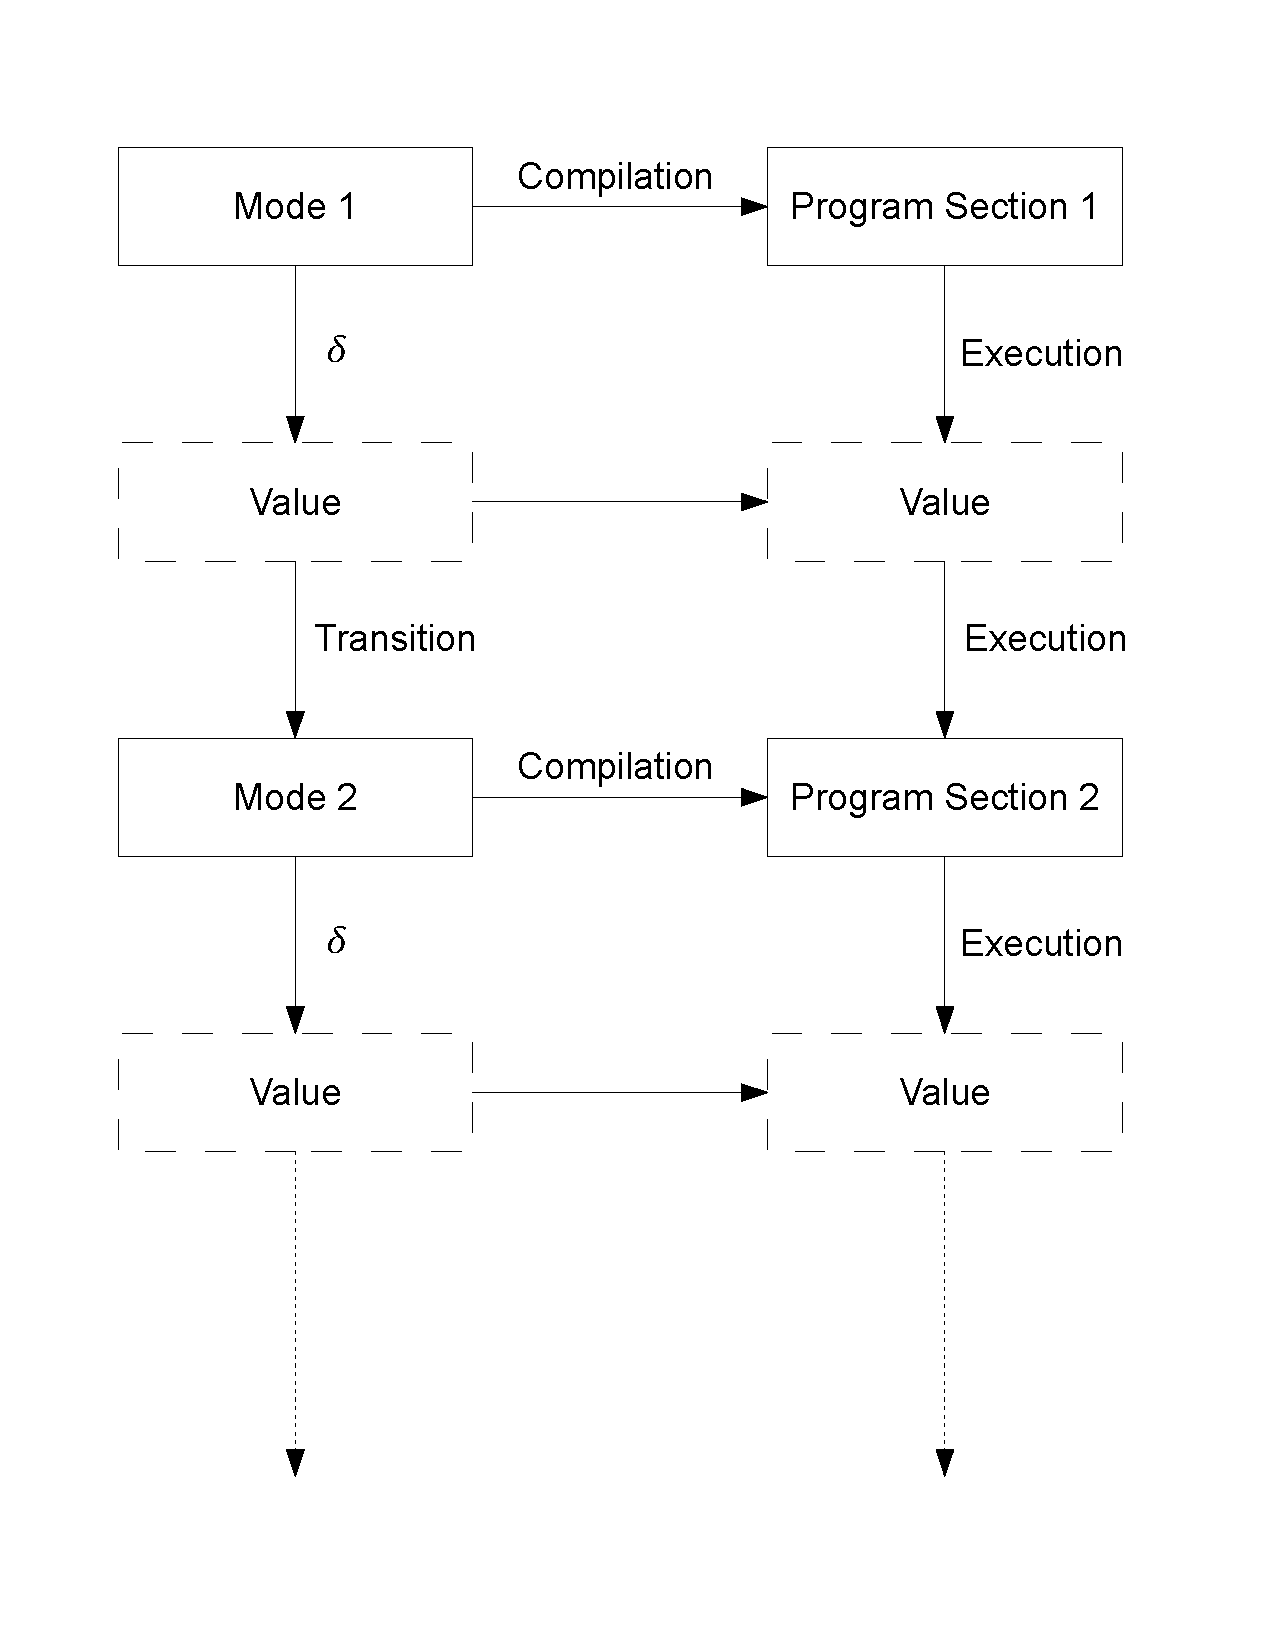
\includegraphics[trim= 10mm 30mm 10mm 10mm, clip, width=\imgmedium]{./images/correctness_graph2.pdf}
    \caption{Code Transition Structure}
    \label{fig:correctness_graph2}
\end{figure}

In this section we will begin by showing that each of the transformations to code are correct examining the basic atoms. We will start by looking at atoms that have the simplest expressions first. The simplest of these is a diagram in which only the start node exists as shown in \ref{fig:correctness_ex_start}.

\clearpage
\subsection{Atoms}

Each block in \plccharts compiles to their own atomic assign statements. In the case were variables are used the type information is not present in the atomic code generation. Variables are collected at compile time declared and initialized as part of the program construction. By collecting variables in this manner a variable with the same name but given two different types can be identified and will cause a compile error. Also the syntax of \plccharts uses ``:='' as an assign where in the final generated code ``='' will be utilized throughout.

\subsubsection{Start Block}

\begin{figure}[h]
	\centering
	
\includegraphics[width=\imgmedphoto]{./images/correctness_atom_start.png}
	\caption{Start Atom}
	\label{fig:correctness_atom_start}
\end{figure}

\begin{lstlisting}[frame=single]
(No atomic assignments or operations in code)
\end{lstlisting}

The start atom is the only atom in our system to not generate any actual code for the atom itself. Instead as the structure section \ref{structure} will show the start atom is used as a place holder so that transitions can be constructed. It also structurally indicates where the program should start.


\subsubsection{Delay Block}

\begin{figure}[h]
	\centering
	
\includegraphics[width=\imgmedphoto]{./images/correctness_atom_delay.png}
	\caption{Delay Atom}
	\label{fig:correctness_atom_delay}
\end{figure}

\begin{lstlisting}[frame=single]
delayms(10);
\end{lstlisting}

The delay atom generates ``delayms($<$expression$>$)''. The expression is the same as in the diagram. The units shown in figure \ref{fig:correctness_atom_delay} as ``ms'' is not included as part of the expression. However the units in the visual representation serves as a reminder that the delay is always measured in milliseconds. Expressions follow the syntax given in the syntax section \ref{sec:statechartsyn} for \plccharts.


\subsubsection{Output Block}

\begin{figure}[h]
	\centering
	
\includegraphics[width=\imgmedphoto]{./images/correctness_atom_output.png}
	\caption{Output Atom}
	\label{fig:correctness_atom_output}
\end{figure}

\begin{lstlisting}[frame=single]
PORTOUT = 0xF2;
\end{lstlisting}

The output atom generated refers to PORTOUT, which is mapped on a hardware level to the PLC hardware implementer's designation of an appropriate output port. This is done to allow the hardware manufacturer a bit of flexability. In our implementation PORTOUT can be assigned any 8-bit value. Any values larger than 8-bit will be trucated. In our example shown in figure \ref{fig:correctness_atom_output} we can see that the assign line diagram is ``PORTOUT := 0xF2''. We can say that the meaning of this line is $\delta(PORTOUT) = 0xF2$. The final compiled output code is ``PORTOUT = 0xF2''. We can see that $Execution(PORTOUT) = 0xF2$ since we have a direct mapping from the value in diagram to value in execution ($\delta(PORTOUT) = Execution(PORTOUT)$). We can conclude that the assignment in the output block is done correctly with respect to the diagram.


\subsubsection{Input Block}

\begin{figure}[h]
	\centering
	
\includegraphics[width=\imgmedphoto]{./images/correctness_atom_input.png}
	\caption{Input Atom}
	\label{fig:correctness_atom_input}
\end{figure}

\begin{lstlisting}[frame=single]
var = PORTIN;
\end{lstlisting}


We can see in figure \ref{fig:correctness_atom_input} that the diagram clearly shows ``int var := PORTIN''. We can say the meaning of the assignment in the diagram is $\delta(var) = PORTIN$. The final compiled code for the atom is ``var = PORTIN''. The left hand side must be a valid variable name as specified in the syntax of \plccharts. The variable can be any type however PORTIN will always be an 8-bit integer, any variable on the left hand side that is not integer would have PORTIN automatically casted to the appropriate type. Thus we can see that $Execution(var) = PORTIN$. We note that there is a direct mapping from digram $value$ to execution $value$, that is: $\delta(var) = Execution(var)$. Thus by our definition of correctness as defined in the beginning of this section and Figure \ref{fig:correctness_graph1}, we can conclude that the input block is correct.


\subsubsection{Store Block}

\begin{figure}[h]
	\centering
	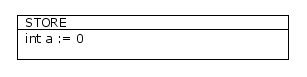
\includegraphics[width=\imgmedphoto]{./images/correctness_atom_store_single.png}
	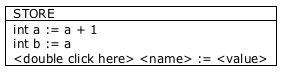
\includegraphics[width=\imgmedphoto]{./images/correctness_atom_store.png}
	\caption{Store Atom}
	\label{fig:correctness_atom_store}
\end{figure}

Single Assign (Left Diagram)
\begin{lstlisting}[frame=single]
a = 0;
\end{lstlisting}

Multiple Assign (Right Diagram)
\begin{lstlisting}[frame=single]
a = a + 1;
b = a;
\end{lstlisting}

The store block is used for assignments. In the left example in figure \ref{fig:correctness_atom_store} we see a store with one assign statement and to the right of figure \ref{fig:correctness_atom_store} we see that store blocks can contain multiple atomic assign statement. 

Looking at the left diagram first we note that the assign statement is ``int a := 0'' that is $\delta(a) = 0$. We see the final generated code is ``$a = 0$'' and $Execution(a) = 0$. We see that $\delta(a) = Execution(a)$ that is to say there exists a mapping from the value in the diagram to the value from execution. We can say that that code generated is correct with respect to the diagram. Looking at the right diagram we see that each line of the store block becomes own atomic assign statements. We see that the diagram has ``int a := a +1'' and ``int b := a'' and by evaluation $\delta(a) = a + 1, \delta(b) = a$. The generated code is then ``a = a + 1'' and ``b = a'' and the executed values $Execution(a) = a + 1, Execution(b) = a$. We can see at this point that $\delta(a) = Execution(a)$ and $\delta(b) = Execution(b)$. Thus we can conclude that the Store Block generated code is correct with respect to our diagram. We note that we can create equivalent store atoms by having two single line store atoms. Thus, it is not difficult to see that the right diagram is just a visual grouping of several atomic assigns for visual simplicity when drawn. Being able to group assigns together into one atomic diagram removes the need to have several atomic assign blocks which ends up being visual noise.


\subsection{Constructors and Transitions}

Aside from atoms compiled code has a few additional constructions. In the example code below we demonstrate the constructed sections for any compiled code. From lines 00-07 is the variable initialization section, any varaibles used are initialized and the type is defined here. Variables in our program are collected at compile time by scanning all the diagram objects and collecting any variables used. Any conflicts between two variable types with the same name are caught and will cause a code generation error at this phase. The initialization section will set all variables to a default value after defning the type.

The generated constructs also provide a way for each of the states to terminate the program if no departing transitions exist. This is accomplished by lines 32-33 ``an end of file'' label is generated to mark the end of the program followed by a return statement to end the program and return control to the programmable logic controller chip. A return statement that exists the program is equivalent to a halt in our case.


\begin{lstlisting}[frame=single]
00 // BEGIN VARIABLE INITIALIZATIONS //
01 int a = 0;
02 int b = 0;
03 float c = 0;
05 double d = 0;
06 char e = 0;
07 // END VARIABLE INITIALIZATIONS //
...
32 EOF:
33 return;
\end{lstlisting}


\clearpage
Transitions are used to string together a sequence of atoms in order to perform the computations necessary in our program. In order to show correctness we must show that the transitions are structurally correct. We must show Transitions will correctly map modes in the right sequence. Figure \ref{fig:correctness_graph2} shows how transitions factor into our overall structure.

\begin{figure}[h]
	\centering
	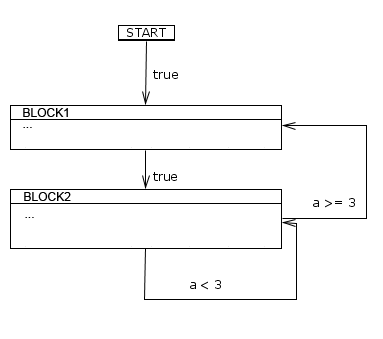
\includegraphics[width=\imgmedphoto]{./images/correctness_ex_transition.png}
	\caption{Transitions}
	\label{fig:correctness_ex_transition}
\end{figure}

%\begin{minipage}{\textwidth}
\begin{lstlisting}[frame=single]
00 // BEGIN VARIABLE INITIALIZATIONS //
01 ...
03 // END VARIABLE INITIALIZATIONS //
04
05 BLUID0:
06 //////////////////////////////////////
07 //        PROGRAM START             //
08 //////////////////////////////////////
09 goto BLUID1;
10 goto EOF;
11
12 BLUID1:
13 //////////////////////////////////////
14 //        BLOCK1                    //
15 //////////////////////////////////////
16 ...
17 
18 goto BLUID2;
19 goto EOF;
20
21 BLUID2:
22 //////////////////////////////////////
23 //        BLOCK2                    //
24 //////////////////////////////////////
25 ...
26
27 if (a >= 3) goto BLUID1;
28 if (a < 3) goto BLUID2;
39 goto EOF;
30
31 EOF:
32 return;
\end{lstlisting}
%\end{minipage}

Starting by looking at the code above we can see that our first entry point into the program is the ``PROGRAM START'' block. This refers to the start block in our diagram. During compilation the entire diagram is scanned to ensure there is one and only one start block. The generated code for the start block is then placed at the top of the program to ensure it is the first entry point of the program after initializers. 

Transitions in our program are compiled to ``goto'' statements. Each block is given a unique ``Block Unique Identifier'' which is a line label starting with ``BLUID''. BLUID's are generated as each block is scanned at compile time and a monotonically increasing number is appended to the end of the label. The ``goto'' transitions always occur after the atomic block assignments have been made.

Looking at diagram \ref{fig:correctness_ex_transition} we note that the start block transitions to ``BLOCK1'' with an edge guarded by ``true''. In the code ``BLOCK1'' has label ``BLUID1'' accociated with it's section of code. We see that the generated code for the start block has a ``goto BLUID1'' on line 9. This corresponds to transition leaving the start block. Next we have a transition from ``BLOCK1'' to ``BLOCK2'' in Figure \ref{fig:correctness_ex_transition}. We can see the code corresponding to the transition on line 18 ``goto BUILD2'' where ``BLUID2'' refers to BLOCK2. Finally we note the two guarded transitions leaving ``BLOCK2''. For the guarded edge ``$a >= 3$'' we can see the generated code ``\texttt{if (a >= 3) goto BLUID1}'' on line 27. We note that ``BLUID1'' refers to ``BLOCK1'' in the diagram so the transition goes from ``BLOCK2'' to ``BLOCK1'' which is correct. For the transition guarded by ``$a < 3$'' we note the generated code on line 28 ``\texttt{if (a < 3) goto BLUID2}''. We see that ``BLUID2'' refers to ``BLOCK2'' so the transition is a self loop, which is correct with respect to the diagram in Figure \ref{fig:correctness_ex_transition}.





%\subsection{Constructors and Compiled Structure}
%\label{structure}
%The construction from atoms to compiled structure follows the constructs outlined in section \ref{sec:implimentation:struct}. Here they are shown in detail in the final compiled form without omissions.
%
%\subsubsection{Start}
%\begin{figure}[htb]
%	\centering
%	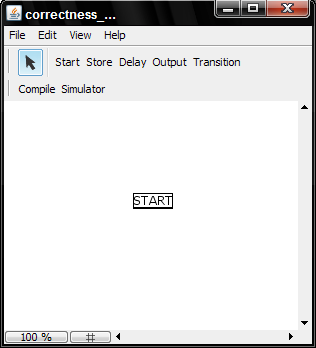
\includegraphics[width=\imgsmall]{./images/correctness_ex_start.png}
%	\caption{Singular Start Block}
%	\label{fig:correctness_ex_start}
%\end{figure}
%In this simple example the following generated intermediate code \emphasize{IL} is created.
%
%\begin{lstlisting}[frame=single]
%00 // BEGIN VARIABLE INITIALIZATIONS //
%01 // END VARIABLE INITIALIZATIONS //
%02
%03 BLUID0:
%04 //////////////////////////////////////
%05 //        PROGRAM START             //
%06 //////////////////////////////////////
%07 goto EOF;
%08 
%09 EOF:
%10 return;
%\end{lstlisting}
%
%In this simplest example we have a label inserted at the beginning of the start block so we can re-enter the start block namely BLUID0. Following the label a comment header to denote the block type, and no variables declared.  Because there is no other transition or block an automatic transition to \emphasize{EOF} is setup in order to terminate the program. In our system this is analogous to ``staying in a state indefinitely'' as the behaviour after return is executed is to just halt the program.
%
%
%\subsubsection{Delay Element}
%
%\begin{figure}[htb]
%	\centering
%	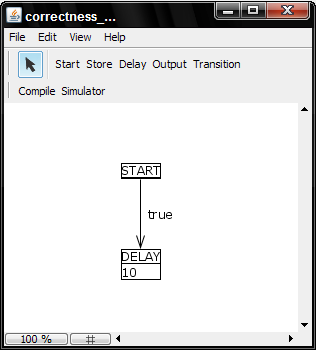
\includegraphics[width=\imgmedsmall]{./images/correctness_ex_delay.png}
%	\caption{Delay Block}
%	\label{fig:correctness_ex_delay}
%\end{figure}
%
%Moving up in complexity we have a start block followed by our next simplest element the delay block, joined by one transition leaving the start block. We can see from figure \ref{fig:correctness_ex_delay}
%the structure of this new graph. We will use this example to examine transitions are compiled into final code, but first we shall look at the delay block itself.
%
%\begin{lstlisting}[frame=single]
%// VARIABLE INITIALIZATIONS //
%...
%
%BLUID1:
%//////////////////////////////////////
%//        DELAY                     //
%//////////////////////////////////////
%delayms(10);
%goto EOF;
%
%EOF:
%return;
%\end{lstlisting}
%
%The delay block itself has a structure identical to the start block. The only difference in this case is the delay block doesn't have a null code section. The delay block generates one line of code, namely delay(integer). The actual delay routine is implemented on the driver level per device since certain devices lack internal timers. It will be up to each implementer to ensure that the delay will correctly delay each the integer specified (in milliseconds). 
%
%\begin{lstlisting}[frame=single]
%00 // BEGIN VARIABLE INITIALIZATIONS //
%01 // END VARIABLE INITIALIZATIONS //
%02 
%03 BLUID0:
%04 //////////////////////////////////////
%05 //        PROGRAM START             //
%06 //////////////////////////////////////
%07 goto BLUID1;
%08 goto EOF;
%09 
%10 BLUID1:
%11 //////////////////////////////////////
%12 //        DELAY                     //
%13 //////////////////////////////////////
%14 delayms(10);
%15 goto EOF;
%16
%17 EOF:
%18 return;
%\end{lstlisting}
%
%In the example shown in figure \ref{fig:correctness_ex_delay} a transition can be seen. The reader will observe that we have directly mapped each edge to a goto statement that is guarded by the guard condition on the edge itself. As defined in section \ref{sec:statechartsyn} the transitions are always mutually exclusive and to not do so would be considered a syntax error. The reason is there is no way to enforce sequence in which each edge is evaluated that would make sense to the programmer constructing the diagram in a visual way. It is up to the programmer (diagram constructor) to ensure that we never run into a condition where two edges actually have an area of overlap. This is not a problem for our simple case as shown in figure \ref{fig:correctness_ex_delay} as we only have one edge leaving the delay block.
%
%Each block has an unique identifier associated with it, this identifier is what is used by the goto blocks in order to recreate the graph structure in the code. The unique identifier is generated at design time and is checked at compile time to ensure that it is in fact unique.
%
%\subsubsection{Output Element}
%
%The output block is similar to the previous delay block however the new item introduced by the output block are variables. The output block during its run will need to set a value to a variable. It does this in order to update the output on the port. 
%
%\begin{figure}[htb]
%	\centering
%	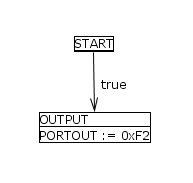
\includegraphics[width=\imgmedphoto]{./images/correctness_ex_output.png}
%	\caption{Output Block}
%	\label{fig:correctness_ex_output}
%\end{figure}
%
%The resulting compiled output from figure \ref{fig:correctness_ex_output} is shown below.
%
%\begin{minipage}{\textwidth}
%\begin{lstlisting}[frame=single]
%00 // BEGIN VARIABLE INITIALIZATIONS //
%01 // END VARIABLE INITIALIZATIONS //
%02 
%03 BLUID0:
%04 //////////////////////////////////////
%05 //        PROGRAM START             //
%06 //////////////////////////////////////
%07 goto BLUID1;
%08 goto EOF;
%09 
%10 BLUID1:
%11 //////////////////////////////////////
%12 //        OUTPUT                    //
%13 //////////////////////////////////////
%14 PORTOUT = 0xF2;
%15 goto EOF;
%16 
%17 EOF:
%18 return;
%\end{lstlisting}
%\end{minipage}
%
%The reader will note that we did not change any of the transitions from figure \ref{fig:correctness_ex_delay}. Despite this the BLUID's are still different. It is easy to see that the ``goto'' routing structure still behaves the same way despite having different labels. We note that the output block's ``set'' operation as shown in figure \ref{fig:correctness_ex_output} becomes translated to ``PORTOUT = 0xF2;'' in the final intermediate language code. The right hand side of the equation can be any valid expression and is not just limited to an costant as shown here. Since the right hand side is transfered verbatim into the final code what the diagram creator draws essentially becomes exactly what is written in the final code.
%
%\subsubsection{Input Element}
%
%Similar to the output block the input block allows you to sample the state of the input ports and store the result into a variable. The first item to the left of the diagram is the variable type. Following the variable type is the variable name. If a new variable name is specified a new entry is created in the variable initialization section. 
%
%
%\begin{figure}[htb]
%	\centering
%	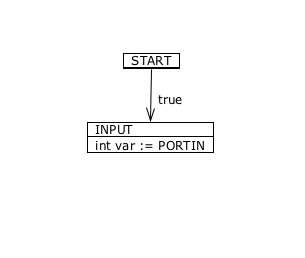
\includegraphics[width=\imgmedphoto]{./images/correctness_ex_input.png}
%	\caption{Input Block}
%	\label{fig:correctness_ex_input}
%\end{figure}
%
%Once again we present the compiled output for \ref{fig:correctness_ex_input} below.
%
%\begin{minipage}{\textwidth}
%\begin{lstlisting}[frame=single]
%00 // BEGIN VARIABLE INITIALIZATIONS //
%01 int var = 0;
%02 // END VARIABLE INITIALIZATIONS //
%03 
%04 BLUID0:
%05 //////////////////////////////////////
%06 //        PROGRAM START             //
%07 //////////////////////////////////////
%08 goto BLUID1;
%09 goto EOF;
%10
%11 BLUID1:
%12 //////////////////////////////////////
%13 //        Input                    //
%14 //////////////////////////////////////
%15 var = PORTIN;
%16 goto EOF;
%17
%18 EOF:
%19 return;
%\end{lstlisting}
%\end{minipage}
%
%Examining the compiled code we will notice that the variable initialization section is no longer empty. Our compiler will first initialize the variable used to store the input from ``PORTIN'' to a known value. This removes any issues of unknown values from our system and as defined in section \ref{sec:statechartsem} variables all have by definition an initial set of values they take on. In the code section of our ``Input'' block we can see that our ``var := PORTIN'' becomes ``var = PORTIN;'' in the final compiled code. The left hand side var is limited to simple variables and expressions are not allowed. Once again like the previous example the data from the input diagram is transfered verbatim into the final code there by ensuring correctness.
%
%\subsubsection{Store Element}
%
%In order to examine transitions in more detail we need to look at logic on transitions. So far because all transitions have been guarded with he condition ``true'' or always taken we have not had the opportunity to see any guard conditions in the code. Instead in the our current code we only observe a always taken goto statement at the end. We will construct a basic diagram with our next component the ``Store Block'' to demonstrate how guard conditions are enumerated as well as demonstrate another basic primitive block that allows the diagram creator to set internal variables and perform calculations.
%
%\begin{figure}[htb]
%	\centering
%	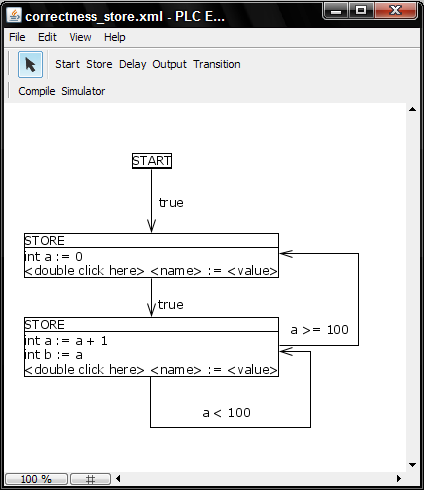
\includegraphics[width=\imgmedphoto]{./images/correctness_ex_store.png}
%	\caption{Store Block Example}
%	\label{fig:correctness_ex_store}
%\end{figure}
%
%The resulting code from figure \ref{fig:correctness_ex_store} is shown below:
%
%\begin{minipage}{\textwidth}
%\begin{lstlisting}[frame=single]
%00 // BEGIN VARIABLE INITIALIZATIONS //
%01 int a = 0;
%02 int b = 0;
%03 // END VARIABLE INITIALIZATIONS //
%04
%05 BLUID0:
%06 //////////////////////////////////////
%07 //        PROGRAM START             //
%08 //////////////////////////////////////
%09 goto BLUID1;
%10 goto EOF;
%11
%12 BLUID1:
%13 //////////////////////////////////////
%14 //        STORE                     //
%15 //////////////////////////////////////
%16 a = 0;
%17 
%18 goto BLUID2;
%19 goto EOF;
%20
%21 BLUID2:
%22 //////////////////////////////////////
%23 //        STORE                     //
%24 //////////////////////////////////////
%25 a = a + 1;
%26 b = a;
%27
%28 if (a >= 3) goto BLUID1;
%29 if (a < 3) goto BLUID2;
%30 goto EOF;
%31
%32 EOF:
%33 return;
%\end{lstlisting}
%\end{minipage}
%
%First we look at the first store block with ``BLUID1'' as its label. We can easily see that from our diagram
%of transformations in figure \ref{fig:correctness_graph1} that our expression ``$a := 0$'' through the compile
%transformation was converted to ``$a = 0$''. Taking the transformation in figure \ref{fig:correctness_graph1}
%of ``$\delta$'' we note that the meaning of ``$a := 0$'' is that the value of $\delta(a) = 0$. Similarily
%executing ``$a = 0$'' in C we find that after execution the value of $exec(a) = 0$. Since the mapping from
%our semantic ``value'' to our executed ``value'' is the same we can conclude that the mapping is correct as
%by our definition. Next we the second store block with ``BLUID2'' as its label. From the diagram in figure
%\ref{fig:correctness_ex_store} the second store block has two notable differences. The first is that it has
%more than one set operation, and the second is that it uses variables in its expression and not just constants.
%As stated before the right hand side allows for any expression to be placed. From our definitions in
%section \ref{sec:statechartsem} of \plcchart it is understood that each expression forumlae is understood
%to occur in sequence. In this example ``$a := a + 1$'' will occur before ``$b := a$''. To demonstrate
%correctness we once again refer to figure \ref{fig:correctness_graph1} and start with our first expression.
%We note that after compilation $a := a + 1$ is compiled to $a = a + 1$, and $b := a$ becomes $b = a$. We
%can see that $\delta(a) = a + 1, \delta(b) = a + 1$, similarly $exec(a) = a + 1, exec(b) = a + 1$. Since
%mapping from $\delta(a) \rightarrow exec(a)$ and $\delta(b) \rightarrow exec(b)$ we can conclude that the
%transformation preserves the meaning of the values and thus is correct to the semantics outlined in
%section \ref{sec:statechartsem}.
%
%To show the correctness of guarded transitions we now look at figure \ref{fig:correctness_graph2}.
%Note that figure \ref{fig:correctness_graph2} shares most of it's structure with
%figure \ref{fig:correctness_graph1} but is annotated to include transitions and modes.
%A mode as established in section \ref{sec:statechartsem} is similar to a state or a block in our diagram.
%Our diagrams always begin from the ``start'' node, similarily our begins its execution from ``BLUID0'' in
%the above code which is the compiled code. No values are updated in our start block so we can take the
%transition leaving the start node this puts us into the first store block (which we will refer
%to as $Store_1$ for disambiguity). On the execution side we see that at the end of the start code
%block we have the line \texttt{goto BLUID1;} we can note that BLUID1 points to the code block for
%our store in the diagram. We can conclude that $Transition(Start, true) \rightarrow Store_1$ similarily
%$Execution(Start, true) \rightarrow Store_1$. Thus we can conclude that transitions leaving ``start'' are
%correct. A similar argument can be made for $Store_1$ since no transitions are guarded.
%
%For the guarded transitions in our second store block which we will refer to as $Store_2$ with
%``BLUID2'' we must look at each guarded condition. We have previously shown for
%figure \ref{fig:correctness_ex_store} that figure \ref{fig:correctness_graph1} holds
%so we will skip showing it again here. Extracting all edges leaving $Store_2$ we
%obtain $Transition(Store_2, a >= 100) \rightarrow Store_1$ and $Transition(Store_2, a < 100) \rightarrow Store_2$.
%Now all that remains is to show that the execution code has the same transitions.
%We can see from the compiled code that at the end of our $Store_2$ code block we have
%a series of ``if'' statements. We can see that \texttt{if (a >= 100) goto BLUID1;} is
%equivalent to $Transition(Store_2, a >= 100) \rightarrow Store_1$ and \texttt{if (a < 100) goto BLUID2;} is
%equivalent to $Transition(Store_2, a < 100) \rightarrow Store_2$. In this way we
%have demonstrated that guarded conditions are correct as well.
%
%By demonstrating that our system is correct both in compilation and the structure execution
%with respect to figures \ref{fig:correctness_graph1} and \ref{fig:correctness_graph2}. We can
%conclude that our system is functionally correct by its construction and structure. To fully
%justify the correctness of the system we still need to show execution traces of each of the
%examples shown in this section. In the next section we will demonstrate execution traces
%of each diagram.


\subsection{Correctness over Execution}
\subsubsection{Table Representation}

In order to show the correctness of the execution it is necessary to identify the differences between graphical traces and execution. Both contain a ``mode'' however in execution the mode can be directly accociated to a set of line numbers. Line numbers don't exist in the diagram view. Both however do have variables and modes, and correct execution is a trace where all modes and variables are identical. To build up our comparison tables we will start with a simple start diagram as shown in Figure \ref{fig:correctness_ex_start}.

\clearpage
\begin{figure}[h]
	\centering
	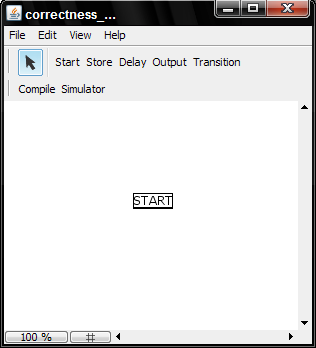
\includegraphics[width=\imgsmall]{./images/correctness_ex_start.png}
	\caption{Singular Start Block}
	\label{fig:correctness_ex_start}
\end{figure}


The accompanying generated \emphasize{IL} code for Figure \ref{fig:correctness_ex_start}.

\begin{lstlisting}[frame=single]
00 // BEGIN VARIABLE INITIALIZATIONS //
01 // END VARIABLE INITIALIZATIONS //
02
03 BLUID0:
04 //////////////////////////////////////
05 //        PROGRAM START             //
06 //////////////////////////////////////
07 goto EOF;
08 
09 EOF:
10 return;
\end{lstlisting}

\begin{table}[htcb]
	\caption{Start Diagram shown in figure \ref{fig:correctness_ex_start}}
	\centering
		\begin{tabular}{| l | l | l | l |}
			\hline
			\textbf{Mode} & \textbf{Variables} & \textbf{Transitions} & \textbf{Next Mode} \\
			\hline
			start & (none) & (none) & (none meaning stop) \\
			\hline
			(none) & (none) & (none) & (none) \\
			\hline
		\end{tabular}
	\label{table:BasicDiagOnly}
\end{table}

To show an execution trace we replace mode with line number and we get the following table.

\begin{table}[htcb]
	\caption{Start code execution for compiled code from diagram \ref{fig:correctness_ex_start}}
	\centering
		\begin{tabular}{| l | l | l | l |}
			\hline
			\textbf{Line} & \textbf{Variables} & \text{Code} & \textbf{Next Executed Line} \\
			\hline
			00 & (none) & (comment) & 07 \\
			\hline
			07 & (none) & \texttt{goto EOF} & 09 \\
			\hline
			09 & (none) & (line label) & 10 \\
			\hline
			10 & (none) & return & (stop) \\
			\hline
		\end{tabular}
	\label{table:BasicExecOnly}
\end{table}

It is not to difficult to see that from lines 00 to 07 we are in the ``start'' mode so we can append a
mode marker to the end of the table. We can also identify that line 09 ``EOF'' represents the end of the
file and thus has no mode accociated with it or goes to a null mode.

\begin{table}[htcb]
	\caption{Start code execution for compiled code from diagram extended\ref{fig:correctness_ex_start}}
	\centering
		\begin{tabular}{| l | l | l | l | l |}
			\hline
			\textbf{Line} & \textbf{Variables} & \textbf{Code} & \textbf{Next Executed Line} & \textbf{Mode}\\
			\hline
			00 & (none) & (comment) & 07 & \textbf{start} \\
			\hline
			07 & (none) & \texttt{goto EOF} & 09 &  \textbf{start}\\
			\hline
			09 & (none) & (line label) & 10 & \textbf{none} \\
			\hline
			10 & (none) & return & (stop) & \textbf{none} \\
			\hline
		\end{tabular}
	\label{table:BasicExecMode}
\end{table}

We can already see that the two traces produce the same outcome however for ease of comparison we can
merge the two tables side by side so we can directly compare each executed line to it's accocated graph.

\begin{table}[htcb]
	\caption{Start code execution combined table. For figure \ref{fig:correctness_ex_start}}
	\centering
	\tablefontsize
		\begin{tabular}{| p{0.06\textwidth} | p{0.1\textwidth} | p{0.15\textwidth} | p{0.06\textwidth} | p{0.05\textwidth} | p{0.1\textwidth} | p{0.2\textwidth} | p{0.07\textwidth} |}
			\hline
			\textbf{Mode} 		&	\textbf{Var (Diag)} 		& 	\textbf{Transitions} 		& 	\textbf{Next}		&	\textbf{Line}		&	\textbf{Var (Exec)	}	&	\textbf{Code}	&	\textbf{Next LN} \\
			\hline
			start 				&	(none)						&	(none)						&	(none meaning stop)	&	00					&	(none)					& 	(comment)		&	07 \\
			\hline
								&								&								&						&	07					& 	(none)					& 	goto EOF		& 	10 \\
			\hline
								&								&								&						&	10					&	(none)					&	return			&	(stop) \\
			\hline
		\end{tabular}
	\label{table:BasicExecCombined}
\end{table}

In table \ref{table:BasicExecCombined} we can easily compare the combined execution vs the diagram code trace. 
We can see that line numbers can be accociated with a mode dispite not having one themselves. In order to verify 
correct execution it is necessary to show that the sequence of modes and values are the same. In the above example
 in which we run our first trivially simple start code snippet it is easy to see that this holds. Therefore we can
  conclude that the execution is correct for the start diagram shown in figure \ref{fig:correctness_ex_start}.

\subsubsection{Start Diagram Execution}

Please see table \ref{table:BasicExecCombined}. We may note that the only mode is ``start'' and that the mode
is followed through the executed line by line trace. We can also note that the code stops after ``start'' 
mode is finished which also is correct behavior. Finally we can note that there are no varibles listed in
our system so both sets of variables are trivially correct.

\subsubsection{Delay Diagram Execution}

\begin{figure}[h]
	\centering
	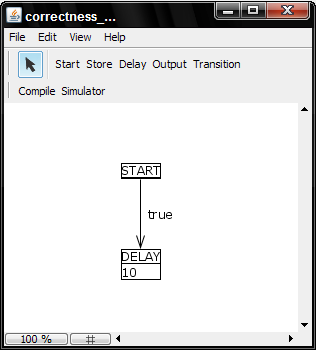
\includegraphics[width=\imgmedsmall]{./images/correctness_ex_delay.png}
	\caption{Delay Block}
	\label{fig:correctness_ex_delay}
\end{figure}

Generated \emphasize{IL} code for diagram in Figure \ref{fig:correctness_ex_delay}.
\begin{lstlisting}[frame=single]
00 // BEGIN VARIABLE INITIALIZATIONS //
01 // END VARIABLE INITIALIZATIONS //
02 
03 BLUID0:
04 //////////////////////////////////////
05 //        PROGRAM START             //
06 //////////////////////////////////////
07 goto BLUID1;
08 goto EOF;
09 
10 BLUID1:
11 //////////////////////////////////////
12 //        DELAY                     //
13 //////////////////////////////////////
14 delayms(10);
15 goto EOF;
16
17 EOF:
18 return;
\end{lstlisting}


\begin{table}[h]
	\caption{Delay code execution combined table. For figure \ref{fig:correctness_ex_delay}}
	\centering
	\tablefontsize
		\begin{tabular}{| p{0.06\textwidth} | p{0.1\textwidth} | p{0.15\textwidth} | p{0.06\textwidth} | p{0.05\textwidth} | p{0.1\textwidth} | p{0.2\textwidth} | p{0.07\textwidth} |}
			\hline
			\textbf{Mode} 		&	\textbf{Var (Diag)} 		& 	\textbf{Transitions} 		& 	\textbf{Next}		&	\textbf{Line}		&	\textbf{Var (Exec)	}	&	\textbf{Code}	&	\textbf{Next LN} \\
			\hline
			start 				&	(none)						&	if (true) delay				&	delay				&	00					&	(none)					& 	(comment)		&	07 \\
			\hline
								&								&								&						&	07					& 	(none)					& 	goto BLUID1		& 	10 \\
			\hline
			delay				&	(none)						&	(none)						&	(stop)				&	10					&	(none)					&	(line label)	&	14 \\
			\hline
								&								&								&						&	14					&	(none)					&	delayms(10)		&	15 \\
			\hline
								&								&								&						&	15					&	(none)					&	goto EOF		&	17 \\
			\hline
								&								&								&						&	17					&	(none)					&	(line label)	&	18 \\
			\hline
								&								&								&						&	17					&	(none)					&	return			&	(stop) \\
			\hline
		\end{tabular}
	\label{table:DelayExecCombined}
\end{table}

Once again in this example we don't have any variable so they are easily verified by checking that in both cases
there are no variables. All that's left to justify correctness is ensuring the sequence of modes is executed correctly.
It should be easy to see that the sequence: start, delay, stop. Is clearly implimented by the executed code from the table
\ref{table:DelayExecCombined}. We can therefor conclude that the excuted code trace is correct with respect to the original
diagram.

\subsubsection{Output Diagram Execution}

\begin{figure}[htb]
	\centering
	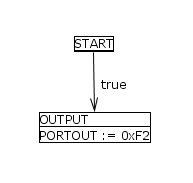
\includegraphics[width=\imgmedsmall]{./images/correctness_ex_output.png}
	\caption{Output Block}
	\label{fig:correctness_ex_output}
\end{figure}

Generated \emphasize{IL} code for diagram in Figure \ref{fig:correctness_ex_output}.
\begin{lstlisting}[frame=single]
00 // BEGIN VARIABLE INITIALIZATIONS //
01 // END VARIABLE INITIALIZATIONS //
02 
03 BLUID0:
04 //////////////////////////////////////
05 //        PROGRAM START             //
06 //////////////////////////////////////
07 goto BLUID1;
08 goto EOF;
09 
10 BLUID1:
11 //////////////////////////////////////
12 //        OUTPUT                    //
13 //////////////////////////////////////
14 PORTOUT = 0xF2;
15 goto EOF;
16 
17 EOF:
18 return;
\end{lstlisting}

\begin{table}[htcb]
	\caption{Output code execution combined table. For figure \ref{fig:correctness_ex_output}}
	\centering
	\tablefontsize
		\begin{tabular}{| p{0.05\textwidth} | p{0.1\textwidth} | p{0.14\textwidth} | p{0.05\textwidth} | p{0.05\textwidth} | p{0.12\textwidth} | p{0.2\textwidth} | p{0.07\textwidth} |}
			\hline
			\textbf{Mode} 		&	\textbf{Var (Diag)} 		& 	\textbf{Transitions} 		& 	\textbf{Next}		&	\textbf{Line}		&	\textbf{Var (Exec)	}	&	\textbf{Code}	&	\textbf{Next LN} \\
			\hline
			start 				&	PORTOUT = 0					&	if (true) output			&	output				&	00					&	PORTOUT = 0				& 	(comment)		&	07 \\
			\hline
								&								&								&						&	07					&   PORTOUT = (no change)	&	goto BLUID		&	10 \\
			\hline
			output				&	PORTOUT = 0xF2				&	(none)						&	(stop)				&	10					&	PORTOUT = (no change)	&	(line label)	&	14 \\
			\hline
								&								&								&						&	14					&	PORTOUT = 0xF2			&	PORTOUT = 0xF2	&	15 \\
			\hline
								&								&								&						&	15					&	PORTOUT = (no change)	&	goto EOF		&	17 \\
			\hline
								&								&								&						&	17					&	PORTOUT = (no change)	&	(line label)	&	18 \\
			\hline
								&								&								&						&	18					&	PORTOUT = (no change)	&	return			&	(stop) \\
			\hline
		\end{tabular}
	\label{table:OutputExecCombined}
\end{table}

First we make a note that PORTOUT is an special variable that is used to send an output to the ports on the device.
According to the hardware specification section PORTOUT is initialized to 0 when the device first starts up.
Likewise PORTOUT is zero until changed in our diagram. In understanding this the rest of the code trace is as follows:
\{(start, PORTOUT = 0), (output, PORTOUT = 0xF2)\} where we observe that our tuple comprises of (mode, variables). 
It is not difficult to see that our two code traces produce this sequence and by our definition we can conclude that our
output execution is correct with respect to the diagram.


\subsubsection{Input Diagram Execution}

\begin{figure}[h]
	\centering
	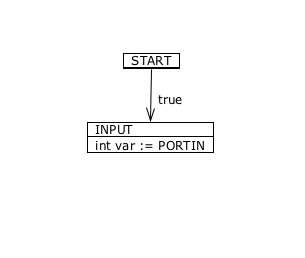
\includegraphics[width=\imgmedsmall]{./images/correctness_ex_input.png}
	\caption{Input Block}
	\label{fig:correctness_ex_input}
\end{figure}

Generated \emphasize{IL} code for the diagram in Figure \ref{fig:correctness_ex_input}.
\begin{lstlisting}[frame=single]
00 // BEGIN VARIABLE INITIALIZATIONS //
01 int var = 0;
02 // END VARIABLE INITIALIZATIONS //
03 
04 BLUID0:
05 //////////////////////////////////////
06 //        PROGRAM START             //
07 //////////////////////////////////////
08 goto BLUID1;
09 goto EOF;
10
11 BLUID1:
12 //////////////////////////////////////
13 //        Input                    //
14 //////////////////////////////////////
15 var = PORTIN;
16 goto EOF;
17
18 EOF:
19 return;
\end{lstlisting}

\begin{table}[htcb]
	\caption{Input code execution combined table. For figure \ref{fig:correctness_ex_input}}
	\centering
	\tablefontsize
		\begin{tabular}{| p{0.05\textwidth} | p{0.1\textwidth} | p{0.14\textwidth} | p{0.05\textwidth} | p{0.05\textwidth} | p{0.12\textwidth} | p{0.2\textwidth} | p{0.07\textwidth} |}
			\hline
			\textbf{Mode} 		&	\textbf{Var (Diag)} 		& 	\textbf{Transitions} 		& 	\textbf{Next}		&	\textbf{Line}		&	\textbf{Var (Exec)	}	&	\textbf{Code}	&	\textbf{Next LN} \\
			\hline			
								&								&								&						&	00					& 	var = UNDEFINED			&	(comment)		&	01	\\
			\hline
								&								&								&						&	01					&	var = 0					&	int var = 0		&	04	\\
			\hline
			start 				&	var = 0						&if (true) $\rightarrow$ input	&	input				&	04					&	var = (no change)		& 	(comment)		&	08	\\
			\hline
								&								&								&						&	08					&	var = (no change)		&	goto BLUID1		&	11	\\
			\hline
			input				&	var = PORTIN				&	(none)						&	(stop)				&	11					&	var = (no change)		&	(line label)	&	15	\\
			\hline
								&								&								&						&	15					&	var = PORTIN			&	var = PORTIN	&	16	\\
			\hline
								&								&								&						&	16					&	var = (no change)		&	goto EOF		&	18	\\
			\hline
								&								&								&						&	18					&	var = (no change)		&	(line label)	&	19	\\
			\hline
								&								&								&						&	19					&	var = (no change)		&	return			&	(stop)	\\
			\hline
		\end{tabular}
	\label{table:InputExecCombined}
\end{table}

We must first note in this code trace that inputs require a variable in order to store
their data. These inputs are intialized at the beginning of the execution where as 
initialization is not required for our diagram since variables always have an initial
value of 0 when first used. Our table starts with line 00, and 01 which initialize 
our variable, we consider this ``house keeping'' and on the left side of our table we
do not consider this process as entering one of our diagram modes. This time the start
mode occurs 3 rows down with corresponding line 04 the execution of the start block 
and diagram is identical to previous examples with the exception of different line numbers.
The sequence of modes and variables is observed as {(start, var = 0), (input, var = PORTIN)}.
We can observed that ``var'' is set to ``PORTIN'' on row 5 in the diagram and in the 
execution the corresponding set occurs on row 6. Dispite the offset caused by the execution
being a less abstract than the diagram the sequence of modes and variables are identical.
Thus according to our definition of correctness we have shown that both diagram
and execution follow the same modes and variable values as well the same sequence
occurence. We can conclude from this that the execution of the input code sample is correct
with respect to the diagram itself.

\clearpage
\subsubsection{Store Diagram Execution}

\begin{figure}[h]
	\centering
	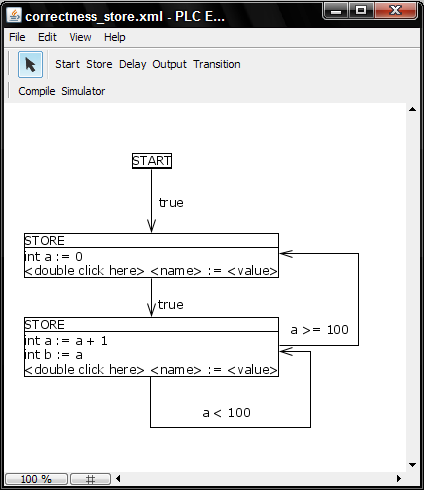
\includegraphics[width=\imgmedphoto]{./images/correctness_ex_store.png}
	\caption{Store Block Example}
	\label{fig:correctness_ex_store}
\end{figure}


Generated \emphasize{IL} code for diagram in Figure \ref{fig:correctness_ex_store}.
\begin{lstlisting}[frame=single]
00 // BEGIN VARIABLE INITIALIZATIONS //
01 int a = 0;
02 int b = 0;
03 // END VARIABLE INITIALIZATIONS //
04
05 BLUID0:
06 //////////////////////////////////////
07 //        PROGRAM START             //
08 //////////////////////////////////////
09 goto BLUID1;
10 goto EOF;
11
12 BLUID1:
13 //////////////////////////////////////
14 //        STORE                     //
15 //////////////////////////////////////
16 a = 0;
17 
18 goto BLUID2;
19 goto EOF;
20
21 BLUID2:
22 //////////////////////////////////////
23 //        STORE                     //
24 //////////////////////////////////////
25 a = a + 1;
26 b = a;
27
28 if (a >= 3) goto BLUID1;
29 if (a < 3) goto BLUID2;
30 goto EOF;
31
32 EOF:
33 return;
\end{lstlisting}


\begin{table}[htcb]
	\caption{Store code execution combined table. For figure \ref{fig:correctness_ex_store}}
	\centering
	\tablefontsize
		\begin{tabular}{|p{0.01\textwidth} | p{0.05\textwidth} | p{0.1\textwidth} | p{0.14\textwidth} | p{0.05\textwidth} | p{0.05\textwidth} | p{0.12\textwidth} | p{0.2\textwidth} | p{0.07\textwidth} |}
			\hline
			\textbf{\#} & \textbf{Mode} 		&	\textbf{Var (Diag)} 		& 	\textbf{Transitions} 		& 	\textbf{Next}		&	\textbf{Line}		&	\textbf{Var (Exec)	}	&	\textbf{Code}	&	\textbf{Next LN} \\
			\hline			
			1&					&								&								&						&	00					& 	a = UNDEFINED \newline	b = UNDEFINED	&	(comment)		&	01	\\
			\hline
			2&					&								&								&						&	01					&	a = 0 \newline b = UNDEFINED	&	int a = 0				&	02	\\
			\hline
			3&					&								&								&						&	02					&	a = 0 \newline b = 0		&	int b = 0					& 	09	\\
			\hline
			4&start				&	a = 0 \newline b = 0		&	if (true) $\rightarrow store_1$	& $store_1$			&	09					&	a = $NC$ \newline b = $NC$	&	goto BLUID1					&	12	\\
			\hline
			5&$store_1$			&	a = 0 \newline b = $NC$		&	if (true) $\rightarrow store_2$ & $store_2$			&	12					&	a = $NC$ \newline b = $NC$	&	(line label)				&	16	\\
			\hline
			6&					&								&								&						&	16					&	a = 0 \newline b = $NC$		&	a = 0						&	18	\\
			\hline
			7&					&								&								&						&	18					&	a = $NC$ \newline b = $NC$	&	goto BLUID2					&	21	\\
			\hline	
			8&$store_2$			&	a = 1	\newline b = 1		&	if ($a \geq 3$) $\rightarrow store_1$ \newline
																	if ($a < 3$) $\rightarrow store_2$ &	$store_2$	&	21					&	a = $NC$ \newline b = $NC$	&	(line label)				&	25	\\
			\hline
			9&					&								&								&						&	25					&	a = 1 \newline b = $NC$		&		a = a + 1				&	26	\\
			\hline
			10&					&								&								&						&	26					&	a = $NC$ \newline b = 1		&		b = a					&	28	\\
			\hline
			11&					&								&								&						&	28					&	a = $NC$ \newline b = $NC$	& if (a \textgreater= 3) goto BLUID1 		&	29	\\
			\hline
			12&					&								&								&						&	29					&	a = $NC$ \newline b = $NC$	& if (a \textless 3) goto BLUID2		&	18	\\
			\hline
			13&$store_2$			&	a = 2	\newline b = 2		&	if ($a \geq 3$) $\rightarrow store_1$ \newline
																	if ($a < 3$) $\rightarrow store_2$ &	$store_2$	&	21					&	a = $NC$ \newline b = $NC$	&	(line label)				&	25	\\
			\hline
			14&					&								&								&						&	25					&	a = 2	\newline b = $NC$	&	a = a + 1					&	26	\\
			\hline
			15&					&								&								&						&	26					&	a = $NC$ \newline b = 2		&	b = a						&	28	\\
			\hline
			16&					&								&								&						&	28					&	a = $NC$ \newline b = $NC$	& if (a \textgreater= 3) goto BLUID1		&	29	\\
			\hline
			17&					&								&								&						&	29					&	a = $NC$ \newline b = $NC$	& if (a \textless 3) goto BLUID2		&	21	\\
			\hline
			18&$store_2$			&	a = 3	\newline b = 3		&	if ($a \geq 3$) $\rightarrow store_1$ \newline
																	if ($a < 3$) $\rightarrow store_2$ &	$store_1$	&	21					&	a = $NC$ \newline b = $NC$	&	(line label)				&	25	\\
			\hline
			19&					&								&								&						&	25					&	a = 3	\newline b = $NC$	&	a = a + 1					&	26	\\
			\hline
			20&					&								&								&						&	26					&	a = $NC$ \newline b = 3		&	b = a						&	28	\\
			\hline
			21&					&								&								&						&	28					&	a = $NC$ \newline b = $NC$	& if (a \textgreater= 3) goto BLUID1		&	12	\\
			\hline
			22&$store_1$			&	a = 0 \newline b = $NC$		&	if (true) $\rightarrow store_2$ & $store_2$			&	12					&	a = $NC$ \newline b = $NC$	&	(line label)				&	16	\\
			\hline
			23&\multicolumn{8}{|c|}{...}\\
			\hline
		\end{tabular}
	\label{table:StoreExecCombined}
\end{table}

The reader should note that we have shortened ``no change'' in the previous tables to ``NC'' in order to fit
in the tables.  Similar to the input example the store example also has variables that must be initialized 
before it can enter it's first state. Lines 00-02 in the table \ref{table:StoreExecCombined} represent the 
``house keeping'' steps required in order to define, setup and initalize the variables. The entry to the start
mode represent the start of our diagram as the reader can see from table \ref{table:StoreExecCombined} the two
variables are considered intitialized to 0 in the diagram, that is ``a = 0, b = 0''. We may also note that this
is taken care in the execution by lines 01 and 02. Thus, line 09 represents the start of our diagram after 
initializations or in the case of diagrams assumptions.

On line 12 we enter our first store block which we
have denoted $store_1$. Observe that only variable ``a'' is modifed in this store block thus ``b'' takes on 
a value of ``NC''. The corresponding operation for ``a = 0'' in the diagram occurs in the execution on line 16.
Finally on line 18 we can see that mode $store_1$ is exited on the execution side by executing ``goto BLUID2''.

On first entry to $store_2$ our diagram updates ``a'' and ``b'' to 1 and 1 respectively, The corresponding line 21 of
the execution is just a line label and the update to variable ``a'' does not occur until line 25. In the generated
code the order of variable assignments is preserved so variable ``a'' is assigned before variable ``b''. Thus, so
far our execution produces the sequence (start, {a=0,b=0}), ($store_1$,{a=0,b=0}), ($store_2$,{a=1,b=1}). We note that
both the diagram and execution produce the same values at this point before continuing.

In the diagram transitions are understood to be evaluated and taken right after the work is done inside the mode.
from table \ref{table:StoreExecCombined} row 8 we can see that the transitions are 
\texttt{if ($a \geq 3$) $\rightarrow store_1$, if ($a < 3$) $\rightarrow store_2$, $store_2$} the result of the
evaluation against a=1 and b=1 is $store_2$. In lines 25-26 we can see the corresponding execution take place to
produced the results for the diagram in row 8. First on line 25 $a = a + 1$ is executed so $a = 0$ that was last set
on row 6 now becomes $a = 1$ after the execution, the following line 26 then sets $b = a$ which is to say $b = 1$ at
this point.

On row 11 we can see that the transitions are now being evaluated. Unlike row 8 on the diagram side where
we treat evaluating transitions as a parallel operation during execution we see that the transitions are evaluated in. 
sequence. Our definition for \plcchart stats that conditions for transitions must be mutually exclusive.
If mutual exclusion was not the case sequence would be important. However, if the conditions are mutually
exclusive it is not difficult to see that regardless of which order each condition is evaluated only a maximum
of one will be true at any point in time. In our case on row 12 $a<3$ is true at this point and we continue to 
execute on the self-loop back into $store_2$.

It is not difficult for the reader to see that row 13 to 17 plays out the same way as 8 to 12 with updates to
variables $a=2, b=2$. We will continue our justification on row 18 were we see that on the diagram side $a=3,b=3$.
We can see that with this condition in place the edge that should be taken according to the diagram is now changed
to $store_1$. We continue to show that the execution trace follows. On line 25 we see that $a=a+1$ updates the 
variable to $a=3$, and line 26 updates $b=a$ making $b=3$. With the variable updated we can now take a look at our
conditions. We can see that $a >= 3$ is now true on line 28 therefore we execute the goto that takes us to $BLUID1$
which is on line 12. This occurs on row 22 of our execution trace.

It is not difficult to see at this point that row 22 is identical to row 5 in both modes and values so they are the
same in our system. This means that our sequence repeates and line 23,24,25... would be identical to 6,7,8... 
respectively. A full execution trace is now (start, {a=0,b=0}), ($store_1$,{a=0,b=0}), ($store_2$,{a=1,b=1},
($store_2$,{a=2,b=2}), ($store_2$,{a=3,b=3}), ($store_1$,{a=0,b=0}), ($store_2$,{a=1,b=1},
($store_2$,{a=2,b=2}), ($store_2$,{a=3,b=3}), ...) repeating forever. We note that both excution and the diagram
were shown to produce this sequence of modes and values, and by our definition we have shown that this 
corresponding code execution is correct with respect to the diagram. 

By showing all executions for all basic atoms in our system we have shown that our system is correct in execution.
All more complex systems can be demonstrated correct in a similar fashion. Because all systems regardless of how
complex are just a combination of atoms any system constructed from these same atoms that are already proved correct,
will also inherently be correct in execution. Thus we can conclude that the execution of this system is then correct
by construction with respect to it's base atoms.